\quiztitle{Geometry}
\quizdescription{Angles, areas, and an isosceles-triangle proof.}
\quizsubject{Geometry}
\quizdifficulty{Intermediate}
\quiztime{18}
\begin{problem}[points=2]
In the triangle shown, find the missing angle in degrees. Enter the number only.
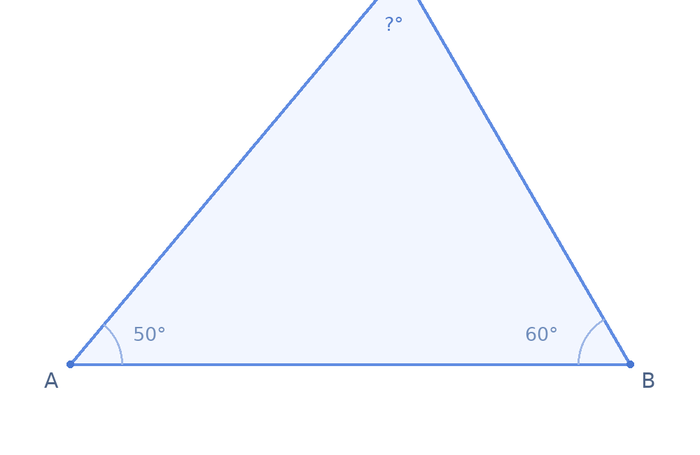
\includegraphics{triangle.png}
\answer{70}
\begin{solution}The interior angles sum to $180^\circ$, so $180-50-60=70$.\end{solution}
\end{problem}
\begin{problem}[points=2]
A right triangle has legs of lengths $6$ and $8$. Find its hypotenuse.
\answer{10}
\begin{solution}By Pythagoras, $c=\sqrt{6^2+8^2}=\sqrt{100}=10$.\end{solution}
\end{problem}
\begin{problem}[points=2]
If the radius of a circle doubles, its area is multiplied by:
\begin{choices}
\choice $2$
\correctchoice $4$
\choice $8$
\choice $\pi$
\end{choices}
\begin{solution}$\pi(2r)^2=4\pi r^2$.\end{solution}
\end{problem}
\begin{problem}[points=3]
Find the area of a circle with radius $3$. You can enter an expression involving pi.
\answer{9*pi}
\begin{solution}$A=\pi r^2=9\pi$.\end{solution}
\end{problem}
\begin{problem}[points=4,mode=manual]
In triangle $ABC$, suppose $AB=AC$. Explain why $\angle B=\angle C$.
\begin{solution}
Let $M$ be the midpoint of $BC$. The triangles $ABM$ and $ACM$ are congruent by SSS, since $AB=AC$, $BM=CM$, and $AM$ is common. Their corresponding angles at $B$ and $C$ are equal.

Marking guide: 1 point for a useful construction, 2 points for a valid congruence argument, and 1 point for the conclusion. Any other complete proof earns 4 points.
\end{solution}
\end{problem}
